\chapter{Análisis Numérico}

\label{ch:numerico}

\section{Principios generales para el tratamiento numérico de bifurcaciones}
Es de suponer por todo lector, tras los ejemplos vistos anteriormente, que estudiar analíticamente las bifurcaciones de sistemas dinámicos con origen biológico se vuelve, en la mayoría de los casos una tarea bastante ardua. Por eso mismo surge, inevitablemente, el estudio numérico de los comportamientos no sólo anteriormente descritos sino, de todos los que de alguna manera se relacionan con la descripción cualitativa de sistemas dinámicos.\\
En particular vamos a introducir en este apartado los conceptos básicos y métodos más utilizados para el estudio cualitativo de algunas de las bifurcaciones del capítulo anterior.\\
En esta exposición vamos a tratar el estudio de sistemas con un parámetro libre, los métodos serán generalizables a distintas disyuntivas. Procedemos de esta manera debido a que exponerlos todos sería a priori una tarea hercúlea y desde un primer momento inabarcable, puesto que para cualquier cambio que se aleje de este marco, supondrá un cambio notable en los métodos (véase \cite{Lectures} y \cite{prac}). Además no hemos de olvidar que nuestro sistema no tiene porqué ser uniparmetrico, lo único que exigimos para este estudio es que el resto de los parámetros estén fijados.
\subsection{Presentación del problema}
Partimos de un sistema dinámico uniparamétrico (o multiparámetro si mantenemos todos los parámetros fijos excepto uno) el cual queremos estudiar cualitativamente. A priori dada la naturaleza de nuestro problema, solemos contar con un rango de valores paramétricos sobre los que realizamos el estudio.\\
Supongamos que el rango de parámetros de interés es $\alpha_a \leq \alpha \leq \alpha_b $. A través de nuestro algoritmo de resolución calcularemos la primera de ella $\alpha_0=\alpha_a$. Como es de suponer este paso en general no será ni inmediato ni sencillo.  
Suponemos por tanto que la solución se puede calcular para  $\alpha_0=\alpha_a$.
Después de haber tenido éxito con  $\alpha_0=\alpha_a$, la siguiente pregunta es cómo elegir  $\alpha_1$.\\Un enfoque útil podemos encontrarlo en los fundamentos de las asignatura de análisis numérico de EDP's. Intuitivamente podríamos pensar que si utilizamos una partición equidistante con una cantidad de nodos cualesquiera (previamente escogidos), obtendríamos de ella una buena manera de elegir el valor de los parámetros subsiguientes de nuestro estudio.
Sin embargo es habitual que usando esta estrategia nos encontremos tres aspectos problemáticos a solventar:
\begin{itemize}
	\item  Se puede pasar por alto una bifurcación.
	\item  Un punto de inflexión o giro ocurre: una bifurcación fold (Figura \ref{diagfold}), y nuestro algoritmo de resolución no funciona adecuadamente.
	\item \textit Aumento del coste computacional: tratar el problema con un espacio muy pequeño puede ocasionar costes elevados.
\end{itemize}
A modo de esquema-resumen, aunque veremos los pasos con más detalle en los siguientes apartados, para paliar las disposiciones más delicadas debemos contar con estas herramientas: \\
Lo primero que necesitamos es \textit{un método de continuación}. Este método genera una cadena de soluciones, además, los candidatos razonables para el incremento de nuestro parámetro son calculados de forma adaptativa. Además el método también puede complementarse con un chequeador de la estabilidad de la rama que estamos estudiando.\\
Por otra parte necesitaremos una forma de detectar y clasificar las bifurcaciones si este método las encuentra.\\
Por último, en muchas ocasiones se puede observar el añadido de un algoritmo que nos permita saltar entre las ramas del diagrama. Es necesario, por tanto, que nuestro método se capaz de calcular distintas ramas de soluciones, pues esto es lo que nos dará una visión acertada global, sin embargo no incluimos aquí la teoría asociada para no extender en demasía el trabajo,  lo que nos permite dar una idea general del método que puede ampliarse con la bibliografía.

\subsection{Cálculo de soluciones iniciales}
Antes de comenzar con los métodos propiamente dichos, me permito profundizar ligeramente en este apartado. En el mismo inicio de nuestro estudio nos encontramos ante este problema:
\begin{equation}
x'=f(x,\alpha_0), x\in\mathbb{R}^n, \alpha\in\mathbb{R},
\end{equation}
de donde queremos obtener las soluciones de la ecuación:
\begin{equation}
0=f(x,\alpha_0), x\in\mathbb{R}^n, \alpha\in\mathbb{R}.
\end{equation}
Es decir, los puntos fijos. A la solución de este problema es a la que le aplicaremos la continuación para obtener el resto de valores. Ahora bien, para ello debemos comenzar con algún valor de nuestro parámetro y, sea cual sea, puede que esta tarea se nos presente muy difícil. Por ello, normalmente, se siguen un par de estrategias éstandar (\cite{Lectures}, \cite{prac}, \cite{siam1} y \cite{graduate}):
\begin{itemize}
	\item Discutir las soluciones de problemas derivados del nuestro de forma que estas sean un caso particular simplificado que nos ayude.
	\item Tomar el rango de valores del parámetro de manera que el primero de ellos simplifique nuestro sistema (en general suele usarse $\alpha_0 =0$).
\end{itemize} 

He de resaltar que en este paso se utiliza un concepto adaptado que nos introdujeron en la asignatura de Topología II: la homotopía. \\
El concepto de homotopía en este contexto surge de la necesidad de resolver una ecuación que a priori se nos presenta difícil. En general el problema no es exclusivo del estudio de bifurcaciones, por lo que, por comodidad notaremos $(x,\alpha)=y$.\\
Supongamos pues que tenemos una expresión de la forma $g(y)=0$ que queremos resolver.
Supongamos que tenemos $f(y)=0$ que es una función sencilla, obtenida de simplificar nuestra $g(y)$ inicial, y que es fácil de resolver. El concepto de homotopía consiste en construir una sucesión de n ecuaciones, que resueltas una a una en orden consecutivo, nos permita llegar a solucionar nuestra ecuación inicial:
\[ f_{0}(y)=f(y)=0\rightarrow f_{1}(y)=0\rightarrow\dots \rightarrow f_{n-1}(y)=0 \rightarrow f_{n}(y)=g(y)=0. \]
La diferencia entre dos términos debe ser lo suficientemente pequeña para que así también lo sea las soluciones asociadas a cada uno.\\
La caracterización anterior no es mas que una versión discreta del proceso de homotopía y, al uso, seguimos teniendo el problema de definir adecuadamente las funciones intermedias. Este escollo lo podemos solventar traduciendo nuestro problema a una formulación continua y, tras ello aplicar métodos de continuación estándar. 
Usemos $0 \leq\lambda\leq 1$ con $\lambda \in \mathbb{R}$ y construyamos una funcion
\begin{equation}
f^{hom}(y,\lambda)=0,0 \leq\lambda\leq 1. 
\label{homotopi}
\end{equation} 
tal que 
\[ f^{hom}(y,0)=f(y) \text{ y } f^{hom}(y,1)=g(y). \]
El problema ahora puede ser la forma de escoger (\ref{homotopi}). Esto es ya sin embargo terreno del estudio de cada problema. Planteamos aquí alguna elección estándar como puede ser:
\begin{equation}
f^{hom}(y,\lambda):=\lambda g(y)+(1-\lambda)f(y).
\label{homotopi2}
\end{equation} 
De hecho soluciones incluso más sencillas (y mucho más complejas) se han encontrado útiles\cite{allgower}.

Es también reseñable como este problema está intrínsecamente relacionado con parte de  nuestro problema inicial, uniendo conceptos que se nos muestran en topología con el cálculo de las ramas de un diagrama de bifurcaciones (presentados en el tema anterior). Este hecho nos muestra como la interconexión de ideas puede ser altamente fructuosa en métodos numéricos.
\subsection{Método de continuación}
Describiremos en esta sección la caracterización método de continuación, así como varios métodos numéricos aplicables en cada caso. Lo haremos desde una perspectiva adaptad a las bifurcaciónes aunque, como veremos, es un método que se puede utilizar para multitud de problemas.
\subsubsection{Planteamiento}
Nuestra intención es estudiar los puntos de equilibrio de un sistema dada la variación de un parámetro. Como sabemos estos puntos vienen determinados (su existencia, no su estabilidad) por la anulación de la función que determina el sistema.\\
Consideremos, pues, un sistema continuo:
\begin{equation}
x'=f(x,\alpha),\text{ } x\in\mathbb{R}^n, \text{ }\alpha\in\mathbb{R}.
\label{formulacionbasica}
\end{equation}
Donde f es una función suficientemente derivable. Los puntos de equilibrio de (\ref{formulacionbasica}) satisfacen
\begin{equation}
f(x, \alpha) = 0.
\label{cero}
\end{equation}
Es decir, un sistema de n ecuaciones escalares en $\mathbb{R}^{n+1}$. Generalmente (\ref{cero}) define una curva (o en cualquier caso una variedad 1-dimensional) $M$, en $\mathbb{R}^{n+1}$. El cálculo de esta
variedad proporciona la dependencia de un equilibrio de (\ref{formulacionbasica}) con respecto al parámetro  de nuestra formulación.\\
El problema de calcular la curva M es el prototipo del caso de estudio de los problemas de continuación:
\begin{equation}
f(x,\alpha)=0,\text{ } f:\mathbb{R}^{n+1}\rightarrow\mathbb{R}^n.
\label{cumplir}
\end{equation}
Por el Teorema de la Función Implícita, el sistema (\ref{cumplir}) define localmente un
curva $M$ que pasa por cada punto $(x_0,\alpha_0)$ que satisface (\ref{cumplir}), siempre que el $rango(J)
= n$, donde $n$ es el número de equaciones que definen el sistema, y $J$, es la matriz jacobiana de (\ref{cumplir}) en $(x_0,\alpha_0)$.\\
La solución numérica del problema de continuación (\ref{cumplir}) nos aportará una sucesión de puntos que nos permitirán aproximar $M$ en mayor o menor exactitud. Habitualmente, utilizando los métodos de resolución convencionales comenzaremos por un $(x_0,\alpha_0)$ lo mas aproximado a $M$ posible. \\Con este fin, se siguen estrategias estándar basadas en hallar un punto de equilibrio a partir del cual comenzar. Fijada habitualmente una homotopía y usando algoritmos de resolución, como el método de Newton, para aproximar este punto inicial. Veremos en el siguiente apartado un estudio más concreto de estos métodos, centrándonos en aquello que usa el software que utilizamos. 

La mayoría de los algoritmos de continuación utilizados en el análisis de bifurcaciones se basan en la implementación de \textbf{Métodos de predicción-corrección} como puede verse en casi todos los libros de esta temática, por citar varios: \cite{Lectures}, \cite{siam1}, \cite{auto}. Estos métodos se componen de tres subetapas que pasamos a describir con mas detalle:
\begin{enumerate}
	\item predicción del siguiente punto,
    \item corrección del punto calculado,
    \item control de tamaño de paso o discretización.
\end{enumerate}

\subsubsection{Predictores}
Comenzamos con la discusión de los predictores. Básicamente los predictores son un mecanismo que nos permiten dar una estimación inicial o \textquotedblleft poco refinada\textquotedblright de lo que será el siguiente par $(x,\alpha_n)$ a estudiar en nuestro problema \ref{cumplir} . Los predictores se pueden dividir en dos clases \cite{prac}:
\begin{itemize}
	\item  Métodos basados en ecuaciones diferencial, es decir que se basan en $f (x, \alpha)$ y sus derivadas.
	\item Métodos basado en extrapolación polinomial, que utiliza sólo soluciones $(x, \alpha)$ de la ecuación (\ref{cumplir}).
\end{itemize}
 En general, para este apartado se suelen utilizar métodos muy estandarizados dejando un poco el refinamiento de estos a la parte de corrección. En nuestro caso vamos a comentar dos de ellos con el fin de mostrar la filosofía de los mismos:
\begin{itemize}
	\item Predictor tangente\\
Tomando la derivada de ambos lados de la ecuación (\ref{cero}), se obtiene
\begin{equation}
0 = df = f_x dx + f_\alpha d\alpha, \label{44}
\end{equation} 

y por lo tanto
\[\frac{dx}{d\alpha}= -(f_x)^{-1}f_\alpha. \]

Integrando este sistema a partir de los valores iniciales $(y_1, \alpha_1)$, se obtiene
la curva $M$ en la que $(y_1, \alpha_1)$ se encuentra. Este procedimiento, propuesto por \cite{georg}, falla en puntos de inflexión debido a la singularidad que se forma en estos puntos por $f_y$. Esto es solventable a través de varias estrategias siendo las más común cambiar el parámetro que estamos evaluando o considerar $x$ y $\alpha$ como funciones dependientes del parámetro arco \cite{prac}.

Esta idea sirve de germen para uno de los predictores más usados. Hablamos del \textbf{Predictor tangente}. Introducimos notación: Sea $z_i = i-esima$ componente de $z$ y, $ z_i = dx_i (1 \leq i \leq n), z_{n+1}= d\alpha$.

Con esta notación podemos transformar (\ref{44}) en la ecuación
\begin{equation}
(f_x | f_\alpha)\cdot z = 0.
\end{equation}
Entiéndase $(f_x | f_\alpha)$ como una matriz de vectores columna adjuntados y, $z$, como un vector tangente.\\
¿Qué podemos decir sobre z? En primer lugar, la recta que contiene al vector es única (aquí estamos asumiendo que $(f_x | f_\alpha)$ tiene rango máximo). Por otra parte el módulo y la orientación del vector z nos son desconocidas. Para obtener una solución única debemos imponer condiciones de normalidad: basta por ejemplo $e. z = 1$ con $e$ algún vector unitario (n+1)-dimensional.\\

En general la formulación de estos métodos puede escribirse como:
\begin{equation}
(x^{j + 1}, \alpha_{j + 1}): = (x^j, \alpha_j) + \sigma_j z_j. \label{normalizao}
\end{equation} 
 Donde $\sigma_j$ es una longitud de paso apropiada. El concepto de apropiedad puede parecernos pernicioso, pero comprobaremos que es habitual que la longitud cambie para adaptarse a nuestro problema (ver \ref{longitud} - Longitud de paso).

Este predictor tangente puede considerarse un paso del método de Euler para resolver una ecuación diferencial que describe la curva $M$, o, lo que es lo mismo, una aproximación de Taylor de orden 1. Por lo tanto, el error de discretización conocido por la asignatura de métodos numéricos II se puede aplicar aquí, obteniendo un error de orden 1.

\item Extrapolación polinomial:\\
Las ideas de extrapolación polinomial también pueden usarse para el paso de predicción. En este caso el método  se basa en la creación de  un polinomio en $\alpha$ de grado $n$ que pasa por los puntos:
\[ (x_j, \alpha_j), (x_{j-1}, \alpha_{j-1}),. . . , (x_{j-n}, \alpha_{j-n}). \]
Si suponemos que este polinomio proporciona una aproximación a $M$ en la región en la que calculamos, un predictor será evaluar la función en  la continuación $\alpha \equiv \alpha_{j + 1}$. 
Usando un polinomio de primer orden ,obtenemos el predictor secante que es la alternativa al predictor tangente (\ref{normalizao}), añadimos también un normalización:
\begin{equation}
Prediccion: ( x_{j + 1}, \alpha_{j + 1}): = (x_j, \alpha_j) + \sigma_j \frac{(x_j - x_{j-1} , \alpha_j - \alpha_{j-1})}{|(x_j - x_{j-1} , \alpha_j - \alpha_{j-1})|}.
\label{secant}
\end{equation}
 Con $\sigma_j$ como longitud de paso y en este caso $z=\frac{(x_j - x_{j-1} , \alpha_j - \alpha_{j-1})}{|(x_j - x_{j-1} , \alpha_j - \alpha_{j-1})|}. $
\end{itemize}
 Es frecuente, como se expone en (\cite{prac}),que  los predictores de orden inferior (tangente, secante) son a largo plazo menos costosos y por lo tanto preferidos. El error de discretización del predictor secante de (\ref{secant}) es del mismo orden que el predictor tangente.\\
 Añadimos además un pequeño esquema para visualizar la diferencia entre ambas en la figura \ref{tangent}.
  \begin{figure}[h]
  	\centering
  	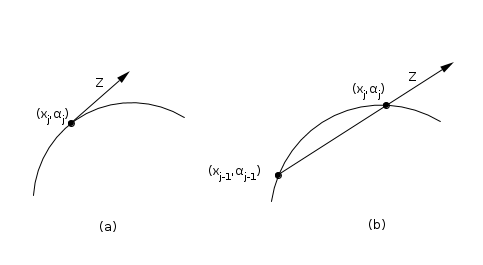
\includegraphics[width=0.7\textwidth]{predic.png}
  	\caption{Representación del predictor tangente (a) y secante (b)}
  	\label{tangent}
  \end{figure}
 En general, la filosofía de estas aproximaciones (debido en parte a que son las más básicas que se usan) ya apareció en la asignatura de métodos numéricos II.
\subsubsection{Correctores}
 Una vez hemos predicho $( x_{j + 1}, \alpha_{j + 1})$, que suponemos suficientemente cercano a nuestra curva, vamos a aplicar un paso para refinar esta predicción y dar con nuestro candidato. Es lo que conocemos como \textbf{Corrección}. Mediante este paso vamos a intentar localizar el que será el siguiente punto de nuestra recta de forma definitiva con una determinada precisión (que impondremos nosotros).
 
 Para este paso normalmente se utilizan técnicas de resolución basadas en el método de Newton, para ello necesitamos el mismo número de ecuaciones que de incógnitas si queremos poder aplicarlo.\\
 La forma habitual de estar seguros de tener el número correcto de ecuaciones es añadir el parámetro mediante el cual vamos a parametrizar nuestra curva $M$. Pues si establecemos nuestra parametrización mediante una ecuación escalar adicional: $g^j(x,\alpha)$ podemos extender el sistema y aplicar así el método de Newton en:
 \[\left\lbrace  \begin{array}{ccc}
 f(x,\alpha)=0,  \\
 g^j(x,\alpha)=0.
 \end{array} \right.
 \]
  De hecho en muchos casos este concepto entiendo puede entenderse geométricamente como intersecar la recta $M$ con una hipersuperficie cercana a nuestro punto. Para facilitar la notación, de nuevo, denotemos $(x,\alpha)=y$, $(x_j,\alpha_j)=y_j$ para el punto definitivo y $(x_j,\alpha_j)=\tilde{y}_j$ para el predicho.
 \begin{itemize}
 	\item \textbf{Continuación por pseudo-longitud de arco }
 	
 	En este caso vamos a seleccionar el hiperplano que pasa por el punto $\tilde{y}_{j+1}$ que es ortogonal al vector $z$, es decir, nuestra funcion corrección estará definida como:
 	\begin{equation}
	g^j(x,\alpha) =\langle y-\tilde{y}_{j+1},z\rangle =\langle y-y_{j},z\rangle-\sigma_j.
	\label{pseudoarco}
 	\end{equation}
 	Si la curva es regular y el tamaño del paso $\sigma_j$ es suficientemente pequeño, se puede probar \cite{Keller}, que las iteraciones de Newton para el sistema formado por el paso de corrección y (\ref{cumplir})  convergerán a un punto $y_{j+1}$ sobre la curva $M$ desde el punto predicho $\tilde{y}_{j+1}$.
 	
 	\item \textbf{Continuación Moore-Penrose} 
 	Mencionamos este caso porque además de ser muy utilizado \cite{allgower} introduce un nuevo cambio al estándar de los pasos de corrección. En cada iteración del método de Newton, nuestra función correctora variará. El plano o curva donde estamos iterando puede hacerse ortogonal a un vector normalizado que satisfaga que el producto escalar de este vector por el jacobiano en el punto anterior sea 0 ($J(Y_{j-i}).V^k=0$) por lo que obtendríamos la siguiente función: 
 		\begin{equation}
 		g^j_k(y) =\langle y-Y_{j + 1},V^k\rangle .
 		\label{moore}
 		\end{equation}
 \end{itemize}

\subsubsection{Longitud de paso}
\label{longitud}
Como se puede esperar hay muchos algoritmos sofisticados para controlar el tamaño del paso $\sigma_j$ \cite{Keller} sin embargo, sorprendentemente uno de los más utilizados, por su fácil implementación y moderada fiabilidad es disminuir el tamaño del paso y repetir las correcciones si no se produce convergencia después de un número prescrito de iteraciones. Si la situación cambia y la convergencia requiere pocas iteraciones aumentamos el tamaño del paso $\sigma_{j + 1}$ con respecto a $\sigma_j$ si la convergencia y, mantenemos el paso actual $\sigma_{j + 1} = \sigma_j$ si la convergencia ocurre después de un número prefijado como aceptable de iteraciones. Esta es la idea básica de los métodos de paso adaptativos, los cuales, como avanzábamos, poseen una literatura enorme.

\subsection{Localización de Bifurcaciones}
Inevitablemente, durante el proceso de construcción de nuestro diagrama de bifurcaciones pasaremos por algunas de ellas. Por tanto para complementar la construcción numérica debemos ser capaces de construir métodos para este fin. 
Supongamos que tenemos una sucesión de soluciones que ha sido aproximada:
\begin{equation}
(x_1, \alpha_1), (x_2, \alpha_2),...
\end{equation}
Supongamos además, que entre dos de ellas: $ (x_{j+1}, \alpha_{j+1})$ y $(x_j, \alpha_j)$ se halla un punto de bifurcación. Nuestro problema será reconocer,  partir de las soluciones, si una bifurcación está cerca.

De nuevo, nos encontramos ante una gran variedad de posibilidades \cite{Kuznet,prac,Lectures} solo copadas por la imaginación de los matemáticos actuales, sin embargo, vamos a introducir aquí una de las más utilizadas que, de hecho, también es la más sencilla.\\
La conclusión sobre si estamos ante un punto de bifurcación vendrá determinada por una función de prueba o función test: $T(x, \alpha)$, que se evalúa durante el proceso de construcción de la curva. Una bifurcación vendrá indicada cuando nuestra función test se anule, es decir:
\begin{defi}
	Una función test para bifurcaciones es una función que satisface la propiedad
	\[T(x_i,\alpha_i)=0\]
	si en $(x_i,\alpha_i)$ hay un punto fijo que experimenta una bifurcación o, convencionalmente, si en $(x_i,\alpha_i)$ hay una bifurcación. Además, es continua en un intervalo suficientemente grande que incluye a $\alpha_i$
	\label{funtest}
\end{defi} 
Los criterios test habitualmente se nos presentan \cite{Lectures,prac}, como una caracterización necesaria, es decir, si nuestra función se anula entonces estaremos ante una bifurcación. Además es usual detectar un punto de bifurcación si nos encontrarnos con un cambio de signo en la función test, puesto que es evidente que tengamos el tamaño de paso que tengamos, sea fijo o variable, no es habitual encontrar el punto exacto.\\ Teniendo esto en cuenta es habitual que nuestro criterio pase a ser:
\begin{equation}
T(x_{j+1}, \alpha_{j+1}) T (x_j, \alpha_j) <0.
\label{crite}
\end{equation}
Puede consultarse en la sección de ejemplos una muestra de aplicación en un caso real \ref{line:sp}.

Una elección temprana, pero igualmente válida puede ser establecer nuestra función test como el máximo de todas las partes reales de nuestros valores propios asociados al jacobiano de nuestro sistema:
\begin{equation}
T:=max\{\Re(\lambda_1),...,\Re(\lambda_n)\}
\label{ftest1}
\end{equation}
Esta función es particularmente significativa puesto que $T<0$ garantizaría estabilidad local. Además si $f(x,\alpha)$ es derivable la función test \ref{funtest} es continua aunque no necesariamente derivable.

Sin embargo, podemos plantear perfectamente el problema de que esta función test no señalará comportamientos si la bifurcación se encuentra en la intersección de dos ramas inestables (ambas partes reales serán negativas). Una buena forma de sobrevenir este problema es modificar nuestra función de partida \cite{funci} y escribirla como:
\begin{equation}
T:=\Re(\lambda_k) \text{ con } |\lambda_k|=min\{|\lambda_1|,...,|\lambda_n|\}
\end{equation}

La función test más utilizada puede obtenerse recurriendo a la propia caracterización de las bifurcaciones fold (o en general de todos puntos donde encontramos una bifurcación), en tanto que en ellas el Jacobiano es singular.:
\begin{equation}
det(f_y(y_0,\alpha_0))=0.
\end{equation}
Teniendo esto en cuenta podemos usar como función test:
\begin{equation}
T(y,\alpha)=det(f_y(y_0,\alpha_0)).
\label{2test}
\end{equation}
Una ventaja que observo de esta función es la conveniencia numérica, pues al realizar la continuación debemos calcular el jacobiano (si seguimos el procedimiento del apartado anterior) y, por tanto, a poco que se piense en la programación del método de Newton, se verá que podemos ahorrarnos el calculo de la función test, aprovechando los residuos del método de Newton.
Típicamente, como vimos en la asignatura de Métodos Numéricos I, el jacobiano puede atacarse a través de la descomposición LU. Así, nuestro jacobiano quedará de la forma:
\begin{equation}
Pf_y=LU
\end{equation}
Donde P es una matriz de permutación. Realizando el determinante en ambas partes:
\[ \pm1  det f_y=1.det U\]
de donde
\[ T= \pm det U \]
Debido a que el determinante de una matriz triangular es igual al producto de los elementos de la diagonal principal, $det U$ y por lo tanto $|T|$ son fácilmente calculables. Aún así debemos prestar atención a tomar el signo correcto de $T$, que depende del de la permutación.

 Como con todas las pruebas de bifurcación, la exactitud de $T$ depende de la precisión con que la que el jacobiano sea evaluado . Además me gustaría destacar que hay dos inconvenientes conocidos para el método \ref{2test}:
 \begin{itemize}
 	\item Evaluar la expresion (\ref{2test}) resulta costosa para sistemas grandes
 	\item El orden de magnitud de (\ref{2test}) puede ser mur grande, esto es: puede resultarnos difícil comparar valores de $T$, por ello, a su vez, ser críticos con tamaños de paso u otros parámetros.
 \end{itemize} 
 
Habitualmente nos encontraremos como a parte de criterios específicos para cada bifurcación, este criterio se incorpora. De nuevo el fragmento de código \ref{line:sp} es un buen ejemplo de ello. Nótese que en ese caso BP hace referencia a Bifurcation Point (criterio para punto de bifurcación).

 Siguiendo la filosofía de la función anterior, es decir, centrarnos en el comportamiento de los valores propios según exista una bifurcación u otra, añado una función test que nos puede ser útil para detectar bifurcaciones de Hopf \cite{Kuznet,prac}:
 \begin{equation}
 T(y,\alpha)_\text{Hopf}=\Pi_{1\leq k<j\leq n}(\lambda_j+\lambda_k)
 \label{3test}
 \end{equation}
 Donde $\lambda$ representa valores propios. Si recordamos la caracterización inicial en el \textit{Capítulo 2} de la bifurcación de Hopf, vemos que en el punto de la bifurcación tendremos dos valores propios imaginarios y complementarios.\\
 Es de destacar que la función test también se anula para valores reales opuestos, por lo que los programas suelen implementar formas de desechar estos datos o directamente utilizar otros métodos mas complejos como las matrices bialternadas en \cite{Kuznet}.
 \subsection{Método de Newton-Chord}
 Para acabar este apartado vamos a presentar la modificación del método de Newton que se presenta en el software que más adelante presentamos.\\
 Como hemos hecho notar a través de la sección anterior es habitual proceder en los métodos de continuación mediante iteraciones tipo Newton. En particular en nuestro caso vamos a destacar el método Newton-Chord.
 Habitualmente no es común poder tener la expresión explicita del Jacobiano, de hecho computacionalmente es una de las partes más costosas (nos referimos aquí al cálculo del jacobiano y de su valor). Por ello multitud de métodos \cite{siam1} se centran en utilizar la filosofía de las iteraciones del método de newton pero evitando el cálculo del Jacobiano. En este marco tenemos la definición del método de Newton-Chord.
 
\begin{defi}[Método de Newton-Chord]
	Sea $x_0$ un número suficientemente cerca de la solución de una ecuación de la forma $F(x)=0$, definimos las \textit{iteraciones del método de Newton-Chord} como:
	\[ x_{n+1}=x_n-F'(x_0)^{-1}F(x_n). \] 
\end{defi}
 
 Es decir, afrontamos el problema del gasto computacional utilizando en todas nuestras iteraciones el Jacobiano (o en $\mathbb{R}^1$, la derivada) calculado en el mismo punto.
 
 Complementario a este apartado, dejamos un resultado, que nos muestra el \textit{precio a pagar} por utilizar este método, es decir, la disminución del orden de convergencia. 
 Dadas las siguientes suposiciones:
 \begin{itemize}
 	\item $F(x)=0$ tiene solución.
 	\item $F':\Omega \rightarrow \mathbb{R}^{N\times N}$ es lipschitciana.
 	\item $F'(x)$ es no-singular.
 \end{itemize}
 \begin{theorem}
 	Existe $\delta>0$ de manera que si $x_0$ pertenece a una bola de centro la solución y radio $\delta$ entonces las iteraciones de Newton-Chord convergen a la solución. Sin embargo:
 	\[ |x_{n+1}-x_{sol}|<k|x_n-x_{sol}| \]
 	para algún $0<k<1$.
 \end{theorem}
 La prueba sigue una filosofía similar al propio método de Newton, puede consultarse en \cite{siam1} para su desarrollo completo. En líneas generales la idea es construir un sistema dinámico discreto con la formulación de las iteraciones. Si este sistema define una aplicación contractiva el Teorema de Punto Fijo de Banach asegura la convergencia. 
 Además, como se puede ver, la convergencia es linear (Newton sin embargo posee convergencia cuadrática, es decir: $|x_{n+1}-x_{sol}|<k|x_n-x_{sol}|^2$ ).
 
 Resaltamos por tanto que métodos que en un principio pueden parecer mejores, se demuestran en la práctica sobrepasados por otros, debido a que, aunque la convergencia tenga menor orden, los cálculos implicados tienen un coste computacional menor.  

 \section{Software utilizado}
 En esta sección recogemos el conjunto del software que recoge las ideas analíticas y numéricas de los capítulos 2 y 3 y, nos sirve para realizar el análisis cualitativo de todos los modelos vistos en el trabajo.\\ Se han utilizado dos herramientas principales para el estudio y una opcional para la visualización dinámica.
 
  \subsection{Python: Diagramas de Fases}
  Pyhton y sus librerías especializadas \cite{Python} se han convertido en toda una referencia para trabajar con matemáticas. Además han permitido dibujar de forma sencilla los resultados y los diagramas de fases de todo éste trabajo.
  
  En librerías como \textit{MatplotLib, SciPy, PySD} ya se encuentran implementados y son fáciles de utilizar.
  Aun así los códigos también son sencillos de implementar por uno mismo. Se puede encontrar el usado en el apéndice.
  
  Aunque el Auto esté fundamentalmente basado en Frotran, son muchas las aportaciones que se le han hecho desde el kernel de Python. Y, aunque aún algo obtusa para trabajar con ella, la próxima alternativa a usar el propio Auto de forma directa vendrá del trabajo en XPPAUT que utiliza en gran medida Python.
  
  \subsection{Geogebra: Visualización dinámica}
  Aunque tiene poca representación en el trabajo, \textit{Geogebra} se ha utilizado para generar visualizaciones dinámicas de forma muy sencilla y que a su vez son también muy visuales. 
  
  Pueden consultarse en el apéndice los códigos utilizados así como alguna imagen de la representación producida.
 
  \subsection{AUTO07-p: Estudio de bifurcaciones}
  Sin duda ha supuesto el gran reto de este trabajo. Si bien es el software de referencia para la creación de diagramas de bifurcaciones, posee una curva de aprendizaje costosísima.
  
  Hay algunos acercamientos desde la comunidad de software libre para suavizar este escollo y ponerse a nivel de software privativo como puede ser MATLAB, que utiliza en su kernel de trabajo código fuente de AUTO07-p, pero posee una interfaz y un sintaxis muchísimo más sencilla.
  
  
  Vamos a hacer un pequeño bosquejo, basándonos fundamentalmente en \cite{auto}, de cómo funciona el intérprete, señalando los archivos necesarios y las etiquetas de las posibles salidas. La interpretación de los resultados, así como  de ciertas etiquetas de los mismos,y, lo que es más importante, la sintaxis habitual del programa, la trataremos en un caso particular, pues entendemos que de esta manera es mucho más sencillo de entender.
  
  Los códigos completos se pueden consultar en los apéndices si se quiere ver una visualización de cómo quedan finalmente.
  
  \subsubsection{Algoritmos utilizados}
  Aunque al ser código libre existe cierta libertad en este aspecto, generalmente, para los problemas de continuación Auto utiliza métodos iterativos basados en Newton-Chord y continuaciones por pseudo-arco. Ambas explicadas en el apartado anterior. \\
  A su vez, como Auto ha recibido numerosas aportaciones y posee más funciones a parte de los algoritmos de continuación, este viene con una gran cantidad de algoritmos diferentes programados a los que se le puede llamar si no queremos que se procesen los específicos.
  
  \subsubsection{Archivo del problema}
  Nos encontramos ante el archivo que describe el problema con las rutinas principales.Este suele acabar con la extensión \textit{.f90}.
  Cada una de las subrutinas viene identificada con una etiqueta, presentamos las que hemos utilizados (para el resto el cuerpo se deja en blanco):
  
  
  \begin{table}[h]
  	\begin{center}
  		\begin{tabular}{|l|l|}
  			\hline
  			FUNC & define la función que vamos a estudiar \\ \hline
  			STPNT & Define la solución inicial y os valores iniciales con los que trabajamos \\ \hline
  			BCND & Define los valores de  frontera \\ \hline
  			
  		\end{tabular}
  		\caption{Datos del archivo de ecuaciones}
  		\label{f90}
  	\end{center}
  \end{table}
  
  
  
  
  
  \subsubsection{Archivo de constantes}
  Es el segundo archivo esencial para el funcionamiento del programa. Normalmente vendrá acompañado de la extensión \textit{.c}.
  En él se definen, nombres, rango de parámetros, dimensión del problema, etc. Dejo en los Cuadros \ref{c} \ref{d} y \ref{t} los datos principales a modo de esquema

 \begin{table}[H]
 	\begin{center}
 		\begin{tabular}{|l|l|}
 			\hline
 			NDIM & Dimensión del sistema \\ \hline
 			NBC & Número de condiciones de contorno (si las hubiera) \\ \hline
 			ISP & Activación de la búsqueda de bifurcaciones  \\ \hline
 			JAC & Según el valor indicamos si se deben especificar las derivadas \\ \hline
 			NINT & Número de condiciones integrales (si las hubiera) \\ \hline
 		\end{tabular}
 		\caption{Tabla constantes del problema}
 		\label{c}
 	\end{center}
 \end{table}
 
 
 
  \begin{table}[h]
  	\begin{center}
  		\begin{tabular}{|l|l|}
  			\hline
  			NTST & Número de intervalos \\ \hline
  			NCOL & Puntos de colocacion de Gauss \\ \hline
  			IAD & Activar o desactivar mallado adaptativo \\ \hline
  		\end{tabular}
  		\caption{Tabla constantes de discretización}
  		\label{d}
  	\end{center}
  \end{table}
 
   \begin{table}[h]
   	\begin{center}
   		\begin{tabular}{|l|l|}
   			\hline
   			EPSL & Critero de convergencia Newton-Chord para parámetros \\ \hline
   			EPSU & Critero de convergencia Newton-Chord para soluciones \\ \hline
   			ITMX & Número máximo de iteraciones \\ \hline
   			NWTN & Criterio de convergencia para el cálculo del jacobiano\\ \hline
   		\end{tabular}
   		\caption{Tabla constantes de tolerancia}
   		\label{t}
   	\end{center}
   \end{table}
 \subsubsection{Salida de datos}
 Como se podrá observar en el siguiente apartado, tenemos dos posibles salidas de datos en nuestro programa.\\
 Una vez ejecutado el código los datos se guardan automáticamente en tres ficheros de extensiones \emph{.b, .d, .s}.
 Además, por una parte, podemos tener la salida por terminal de los datos numéricos (la interpretación de las etiquetas de la misma puede consultarse en el Cuadro \ref{dd}). O también podemos ejecutar el visor gráfico de Auto a través de \begin{lstlisting}
@pp.
 \end{lstlisting}
  En este caso Auto nos mostrará por pantalla una representación gráfica de los datos almacenados. Sin embargo comentar ésta requiere comentar cada caso en particular.
 
 \begin{table}[h]
 	\begin{center}
 		\begin{tabular}{|l|l|}
 			\hline
 		    TY & Tipo de punto \\ \hline
 			BR & Número de rama/curva del diagrama \\ \hline
 			LAB & Etiqueta del punto \\ \hline \hline 
 			BP & Punto de bifurcación\\ \hline
 			HB & Bifurcación de Hopf\\ \hline
 			LP & Bifurcación fold\\ \hline
 			EP & Punto de comienzo\\ \hline
 			MX & Terminación anormal\\ \hline
 			
 		\end{tabular}
 		\caption{Etiquetas de salida de datos}
 		\label{dd}
 	\end{center}
 \end{table}
 
\subsection{Ejemplo completo guiado: Competición entre especies}
Vamos a tratar un caso de competición entre dos especies con roles de presa y depredador \cite{doedel}. Comenzaremos con la descripción matemática del mismo. Analizaremos matemáticamente con sería un diagrama de bifurcaciones y, con a la vista de estos resultados, escribiremos el código necesario para crear el diagrama numéricamente y compararemos los resultados.

 El modelo viene representado por el siguiente sistema:
\begin{equation}
\left \{ \begin{matrix} x'=3x(1-x)-xy-\alpha(1-e^{-5x})\\ y'=-y+3xy \end{matrix}\right .
\label{pp2}
\end{equation}


donde $x$ representarán la presa e $y$ a los depredadores. Además el sistema posee una perturbación en la que las presas son extraídas del sistema ( defunciones, vertidos contaminantes para la especie, o explotación de recursos mediante caza o pesca, etc).

Con $ \alpha=0$ hallamos las soluciones estacionarias :
\[ \left \{ \begin{matrix} 3x(1-x)-xy=0\\ -y+3xy=0  \end{matrix}  \right \} \Rightarrow (x,y)=(0,0),(1,0),(1/3,2) \]
En adelante asociaremos los valores con \emph{a}$=(0,0)$, $b=(1,0)$ y $c=(1/3,2)$. La letra indicará sobre qué valor estamos trabajando.  
La matriz del jacobiano vendrá determinada por
 \[ \left (\begin{matrix} 3-6x-y-5\alpha e^{-5x} && -x \\ 3y && 1+3x  \end{matrix}  \right )=J_{x,y}(x,y,\alpha)\]
 Y, estudiar la estabilidad nos resulta en:
 \begin{enumerate}[a)]
 	\item  \[ \left (\begin{matrix} 3 && 0 \\ 0 && -1  \end{matrix}  \right )=J_{x,y}(0,0,0)\]
 	\item  \[ \left (\begin{matrix} -3 && -1 \\ 0 && 2  \end{matrix}  \right )=J_{x,y}(1,0,0)\]
 	\item  \[ \left (\begin{matrix} -1 && -1/3 \\ 6 && 0  \end{matrix}  \right )=J_{x,y}(1/3,2,0)\]
 \end{enumerate}
cuyos valores propios son:
\begin{enumerate}[a)]
	\item 3, -1, inestable
	\item -3, 2, inestable
	\item $(-1-\lambda)(-\lambda)+2=0;
	\lambda_\pm = \frac{-1\pm \sqrt{-7}}{2}$ La parte real es menor que cero, por tanto estable.
\end{enumerate}

Todos los Jacobianos son no singulares para $\alpha = 0$
En este caso podemos calcular todas las ramas del diagrama de bifurcaciones ( las que hemos llamado $M$):
\begin{enumerate}[a)]
	\item $(x,y)=0$
	\item $y=0$ ;  $ \alpha=\frac{3x-3x^2}{1-e^{-5x}}
	 $ (Nótese que $ \lim_{x\rightarrow 0}\alpha=3/5$)
	\item $x=1/3$ ; $2/3-1/3y-\alpha(1-e^{-5/3})=0 \Rightarrow y=2-3\alpha(1-e^{-5/3})$
\end{enumerate}
Estudiamos la estabilidad de las ramas: 
 \begin{enumerate}[i)]
 	\item  \[ \left (\begin{matrix} 3-5\alpha && 0 \\ 0 && -1  \end{matrix}  \right )=J_{x,y}(0,0,\alpha)\]
 	\item  \[ \left (\begin{matrix} -3-5\alpha e^{-5} && -1 \\ 0 && 2  \end{matrix}  \right )=J_{x,y}(1,0,\alpha)\]
 	\item  \[ \left (\begin{matrix} -1-5\alpha e^{-5/3} && -1/3 \\ 6 && 0  \end{matrix}  \right )=J_{x,y}(1/3,2,\alpha)\]
 \end{enumerate}
tendremos por tanto:
\begin{enumerate}[i)]
	\item Valores propios= $-1$, $3-5\alpha$
	
	de aquí podemos deducir que la solución trivial será inestable si $\alpha<3/5$ y estable en caso contrario, hecho que podremos observar en  la simulación.
	\item No hay estabilidad en esta rama (estamos considerando la variables positivas)
	\item Cuando $\alpha$ se aproxima a $0.67$, tendremos un salto sobre el eje imaginario de los valores propios, es decir, tendremos una bifurcación de hopf.
\end{enumerate}
Concluido el desarrollo analítico, implementamos el código en el programa.

\subsubsection{Creación del código}
Tras el estudio del modelo con herramientas analiticas vamos a ver como podemos aplicar paso a paso las herramientas de programación para obtener el diagrama de bifurcaciones y comprobar nuestros resultados. 
Como comentábamos, AUTO posee muchas variables personalizables, algunas no las vamos a cubrir en los comentarios por centrarnos en las que afectan y definen nuestro problema, pero todas pueden consultarse en el manual \cite{auto} si hay algún tipo de duda.
 
Construimos, en primer lugar, nuestro fichero \textit{nombre-de-programa.f90} e incluimos las dos primeras subrutinas:

\begin{enumerate}
	\item Introducimos las ecuaciones que conforman el sistema \ref{pp2}. Los valores como la dimensión(NDIM), se incorporarán en el archivo de constantes. 
	\begin{lstlisting}[language=Python]
	SUBROUTINE FUNC(NDIM,U,ICP,PAR,IJAC,F,DFDU,DFDP) 

	IMPLICIT NONE
	INTEGER, INTENT(IN) :: NDIM, IJAC, ICP(*)
	DOUBLE PRECISION, INTENT(IN) :: U(NDIM), PAR(*)
	DOUBLE PRECISION, INTENT(OUT) :: F(NDIM)
	DOUBLE PRECISION, INTENT(INOUT) :: DFDU(NDIM,*), DFDP(NDIM,*)
	
	DOUBLE PRECISION e
	
	e=EXP(-PAR(3)*U(1)) 
	
	F(1) = PAR(2)*U(1)*(1-U(1)) - U(1)*U(2) - PAR(1)*(1-e) 
	F(2) = -U(2) + PAR(4)*U(1)*U(2) 
	
	END SUBROUTINE FUNC
	\end{lstlisting}
	
	\item Justo después introducimos las condiciones iniciales y los valores iniciales de nuestros parámetros.
	\begin{lstlisting}[language=Python]
	SUBROUTINE STPNT(NDIM,U,PAR,T)  
	
	IMPLICIT NONE
	INTEGER, INTENT(IN) :: NDIM
	DOUBLE PRECISION, INTENT(INOUT) :: U(NDIM), PAR(*)
	DOUBLE PRECISION, INTENT(IN) :: T
	
	PAR(:4) = (/ 0.0, 3.0, 5.0, 3.0 /)
	U = 0.0
	
	END SUBROUTINE STPNT
	
	\end{lstlisting}
	
\end{enumerate}


Vamos a editar ahora el archivo de constantes. Esta parte no tiene tanta relación con la programación en sí misma. Es habitual encontrar ficheros con el código ejecutable en python o el fichero de las ecuaciones, sin embargo se deja que seamos nosotros los que elijamos los valores concretos de nuestro problema.
El archivo de constantes admite dos formatos, habitualmente se encuentra identificando valores con variables de esta forma:
\begin{lstlisting}[language=Python]
2 1 0 0  NDIM,IPS,IRS,ILP
\end{lstlisting}
Sin embargo para que sea más fácil identificarlo en este ejemplo guiado utilizaremos signos de igualdad para que se puedan identificar más fácilmente los valores. Por supuesto, todas las líneas se escriben una tras otra en el mismo fichero:


Dimensión del problema.
\begin{lstlisting}[language=Python]
NDIM=2
\end{lstlisting}
 Identificación de las variables de salida.
\begin{lstlisting}
unames={1: 'presa', 2: 'depredador'}
parnames={1: 'alpha', 9: 'presa'}
\end{lstlisting}
Imprimir por pantalla y guardar datos cada 100 cálculos.
\begin{lstlisting}
NPR=100
\end{lstlisting}
 Parámetro libre.
\begin{lstlisting}
ICP=['alpha']
\end{lstlisting}
 Límites de las variables y límite de iteraciones.
\begin{lstlisting}
UZSTOP={'alpha': [0.0, 1.0], 'presa': -0.25}, NMX=100
\end{lstlisting}
 Constantes de computación: Tipo de problema (EDO) y etiqueta de la primera solución.
\begin{lstlisting}
IPS=1, IRS=0
\end{lstlisting}
 Tamaño de la discretizacion
\begin{lstlisting}
DS=0.02, DSMIN=0.01, DSMAX=0.06
\end{lstlisting}
 Intervalos
\begin{lstlisting}
NTST=90
\end{lstlisting}

\subsubsection{Ejecución del código} 
Una vez que tenemos los códigos, ejecutamos el comando para entrar en el programa:
\begin{lstlisting}
>AUTO

Python 2.7.12 (default, Nov 19 2016, 06:48:10) 
[GCC 5.4.0 20160609] on linux2
Type "help", "copyright", "credits" or "license" for more information.
(AUTOInteractiveConsole)
\end{lstlisting}

Nos movemos a la carpeta que contiene los ficheros y ejecutamos, bien el archivo python en el que tenemos escritas las órdenes o directamente el archivo de ecuaciones. La forma habitual de hacer esto último es mediante los comandos:
\begin{lstlisting}
cd carpeta_con_nuestro_codigo
nombre_del_archivo = run('nombre_del_archivo')
save('nombre_del_archivo')
\end{lstlisting}

Una vez ejecutado el código, el programa genera varias clases de archivos y presenta los datos por pantalla. Mientras que los archivos generados poseen el registro de salida y la información numérica (los valores de todas las variables que intervienen en nuestro análisis y las generadas mediante el procedimiento numérico), por pantalla se nos muestra un resumen de la información más relevante. En ese caso: 

\begin{lstlisting}
BR    PT  TY  LAB     alpha       L2-NORM         presa         predador    
1     1  EP    1   0.00000E+00   0.00000E+00   0.00000E+00   0.00000E+00
1    12  BP    2   6.00000E-01   0.00000E+00   0.00000E+00   0.00000E+00
1    19  UZ    3   1.00000E+00   0.00000E+00   0.00000E+00   0.00000E+00

BR    PT  TY  LAB     alpha       L2-NORM         presa         predador    
2    21  BP    4   8.21904E-01   3.33333E-01   3.33333E-01   0.00000E+00
2    25  LP    5   8.32929E-01   4.11162E-01   4.11162E-01   0.00000E+00
2    79  UZ    6   2.52388E-06   9.99999E-01   9.99999E-01   0.00000E+00

BR    PT  TY  LAB     alpha       L2-NORM         presa         predador    
2    10  UZ    7   3.76454E-01   2.50000E-01  -2.50000E-01   0.00000E+00

BR    PT  TY  LAB     alpha        L2-NORM        presa         predador    
3    12  UZ    8   1.00000E+00   5.46739E-01   3.33333E-01  -4.33373E-01

BR    PT  TY  LAB     alpha        L2-NORM         presa        predador    
3    10  HB    9   6.71594E-01   4.94866E-01   3.33333E-01   3.65762E-01
3    40  UZ   10   1.25990E-09   2.02759E+00   3.33333E-01   2.00000E+00

Total Time    0.546E-01
\end{lstlisting}

Si atendemos a BR podemos ver que se han encontrado 3 ramas. Tenemos también todo los puntos que se han encontrado, con la información de los valores de las variables y de $\alpha$. Además tenemos la clasificación del tipo de punto. En la tabla \ref{a} se pueden observar mejor estas etiquetas junto con la tabla \ref{tabla tipo pnto}

Antes de pasar a las gráficas vamos a echar un vistazo a una sección del registro de salida del programa:
\begin{lstlisting}[escapechar=|]

BR    PT  IT         PAR           L2-NORM
3     9   0        6.92629E-01   4.58333E-01
3     9   1        6.92629E-01   4.58333E-01

3     9         Fold Function:   3.80107E-01
3     9         BP   Function:   1.65520E+00
3     9         Hopf Function:   1.56604E-02

3     9         Eigenvalues  :   Stable:   0
3     9         Eigenvalue  1:   1.56604E-02  -5.60652E-01
3     9         Eigenvalue  2:   1.56604E-02   5.60652E-01 |\label{line:sp}|

===============================================

BR    PT  IT         PAR           L2-NORM
3    10   0        6.69822E-01   4.98061E-01
3    10   1        6.69822E-01   4.98061E-01

3    10         Fold Function:   3.80107E-01
3    10         BP   Function:   1.94720E+00
3    10         Hopf Function:  -1.31890E-03

3    10         Eigenvalues  :   Stable:   2
3    10         Eigenvalue  1:  -1.31890E-03  -6.08334E-01
3    10         Eigenvalue  2:  -1.31890E-03   6.08334E-01

\end{lstlisting}

Como se puede comprobar hemos escogido la correspondiente a los datos de la tercera rama calculada, en particular los cálculos correspondientes al paso del noveno punto al décimo.

 Como se puede observar en el registro están los datos de los valores propios y de las funciones test. Hemos querido resaltar éste a modo de ejemplo de como actúan las funciones test de bifurcaciones en un caso practico. Como se puede observar tenemos un cambio de signo en la función, esto se debe al cruce por el eje imaginario de los valores propios (apreciable por el cambio de signo de la primera componente delos valores propios), tenemos por tanto la localización de una bifurcación de Hopf HB, que se marca en la salida por pantalla como:
 \begin{lstlisting}
BR    PT  TY  LAB     alpha        L2-NORM         presa        predador    
3    10  HB    9   6.71594E-01   4.94866E-01   3.33333E-01   3.65762E-01
 \end{lstlisting}


 Finalmente podemos obtener un diagrama de bifurcaciones enfrentando x con el parámetro.
 Evidentemente el diagrama es incompleto, necesitaríamos un gráfico en 3D para poder visualizar correctamente el concepto. Aún así podemos observar que tenemos una bifurcación de Hopf en el valor predicho, o más bien, que nuestro diagrama coincide con una proyección del diagrama en 3D de una bifurcación de hopf. Llegados a este punto se puede afirmar que la población de presas puede regularse mediante los parámetros para que experimente una evolución cíclica, sin embargo traspasar este ciclo podría desencadenar una extinción.
  \begin{figure}[h]
  	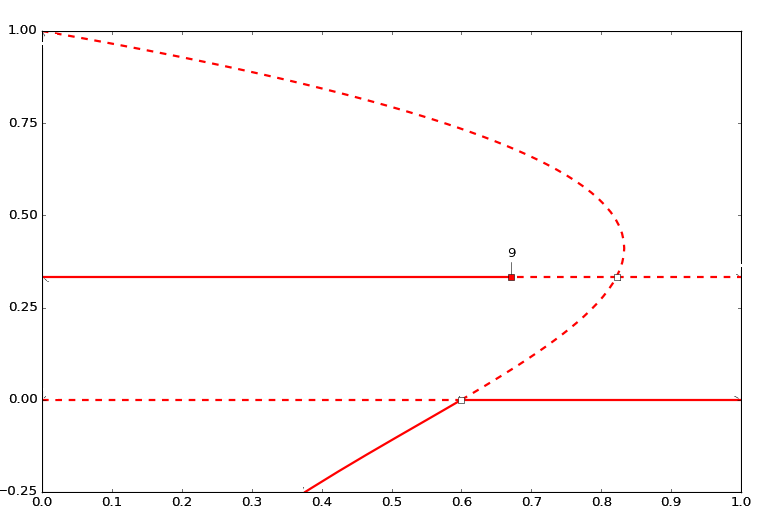
\includegraphics[width=\textwidth]{pp21.png}
  	\caption{Diagrama de bifurcaciones $x-\alpha$ final.}
  \end{figure}
  
\section{Otros diagramas de bifurcaciones}

En este último apartado vamos a representar un par de modelos relacionados con los estudiados en el tema 2.

\subsection{Van der Pol}

En lo que a osciladores se refiere hemos estudiado las cualidades del modelo éstandar. Sin embargo debido a la precisión que requiere el uso de programas como AUTO, vamos a tratar en este apartado una modificación del mismo. Cualitativamente ambos presentan una bifurcación de Hopf con una evolución similar.
Presentamos el modelo:

\begin{equation}
\left \{ \begin{matrix} x'=y-(\frac{1}{3}x^3)-x\\ y'=\epsilon(\alpha-x)\end{matrix}\right . .
\end{equation}  

Como se puede comprobar es una variación del modelo \ref{vanderpol2} en la que optamos por fijar nuestro parámetro en 1 y añadir dos parámetros.El denotado por $\epsilon$ lo fijaremos con antelación y moveremos el parámetro $\alpha$. 

En estos casos, tanto la aplicación de nuestro criterio como la visualización gráfica nos dejan entreveer la aparición de una bifurcación de Hopf.
Por tanto procedemos a escribir el código correspondiente en AUTO y ejecutarlo.

En primer lugar tenemos la salida por pantalla que nos proporciona la verificación de la existencia de una bifurcación de Hopf (mostramos el extracto):

\begin{lstlisting}
BR    PT  TY  LAB    PAR(2)        L2-NORM         
1    16  HB    2   1.00000E+00   1.20185E+00   1.00000E+00  -6.66667E-01
\end{lstlisting}

Y posteriormente, para un análisis completo, podemos usar un visualizador como XPPAUT (código en el apéndice) cuyo núcleo para representar bifurcaciones es AUTO, para visualizar gráficamente los datos: \ref{vandedia}.


 \begin{figure}[h]
 	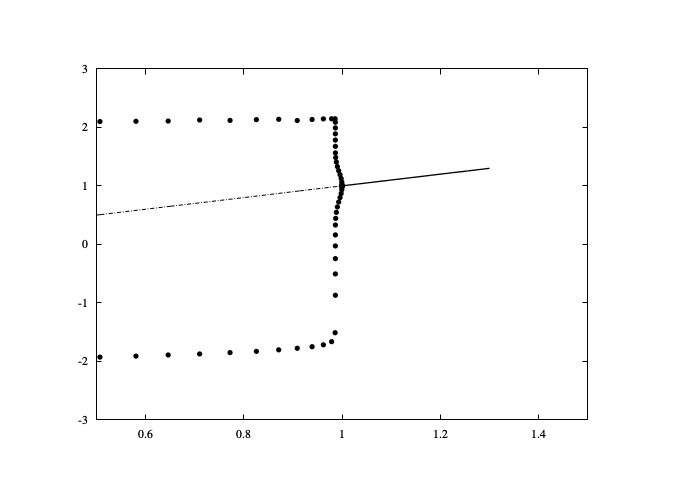
\includegraphics[width=\textwidth]{diagramfinalfinal.png}
 	\caption{Diagrama de bifurcaciones para el modelo \ref{vanderpol}, ejes:  $x-\alpha$ }
 	\label{vandedia}
 \end{figure}

\subsection{Gusanos de las píceas.}

Para completar el trabajo, como el modelo de Sel'kov también experimenta una bifurcación de Hopf, preferimos representar el diagrama de bifurcación fold que experimenta el modelo de ecología \ref{gusaca}.

Este diagrama no es un diagrama \ref{gusacaca}  de bifurcación fold propiamente dicho, pues existen 3 puntos fijos en nuestro sistema. Sin embargo, es apreciable como si nos fijamos en las dos ramas superiores observamos lo que si se corresponde con un diagrama de bifurcación fold. Esto corresponde unívocamente con nuestro problema. 

De nuevo en este caso hemos recurrido a un recurso electrónico para el dibujo, aún así los ficheros con las ecuaciones se adjuntan en el apéndice y pueden ser consultados.

 \begin{figure}[h]
 	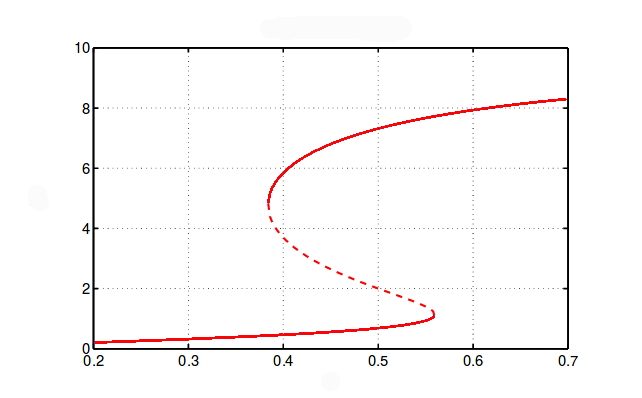
\includegraphics[width=\textwidth]{diagramagusanos.png}
 	\caption{Diagrama de bifurcaciones para el modelo \ref{gusaca}, ejes: $x-r$}
 	\label{gusacaca}
 \end{figure}







